%%%%%%%%%%%%%%%%%%%%%%%%%%%%%%%%%%%%%%%%%
% Simple Sectioned Essay Template
% LaTeX Template
%
% This template has been downloaded from:
% http://www.latextemplates.com
%
% Note:
% The \lipsum[#] commands throughout this template generate dummy text
% to fill the template out. These commands should all be removed when 
% writing essay content.
%
%%%%%%%%%%%%%%%%%%%%%%%%%%%%%%%%%%%%%%%%%

%----------------------------------------------------------------------------------------
%	PACKAGES AND OTHER DOCUMENT CONFIGURATIONS
%----------------------------------------------------------------------------------------

\documentclass[12pt]{article} % Default font size is 12pt, it can be changed here
\usepackage[margin=1in]{geometry} % Required to change the page size to A4
\geometry{a4paper} % Set the page size to be A4 as opposed to the default US Letter

%\usepackage{graphicx} % Required for including pictures
\usepackage{graphicx}
\usepackage{subfig}

\usepackage{float} % Allows putting an [H] in \begin{figure} to specify the exact location of the figure
\usepackage{wrapfig} % Allows in-line images such as the example fish picture

\usepackage{lipsum} % Used for inserting dummy 'Lorem ipsum' text into the template

\usepackage{pdfpages}

\usepackage{enumitem}

\usepackage[nottoc,numbib]{tocbibind}

\bibliographystyle{abbrv}

\usepackage[toc,page]{appendix}

\linespread{1} % Line spacing

%\setlength\parindent{0pt} % Uncomment to remove all indentation from paragraphs

\graphicspath{{Pictures/}} % Specifies the directory where pictures are stored

% Commands
\newcommand{\HRule}{\rule{\linewidth}{0.5mm}} % Defines a new command for the horizontal lines, change thickness here


\begin{document}

%----------------------------------------------------------------------------------------
%	TITLE PAGE
%----------------------------------------------------------------------------------------

\begin{titlepage}

\center % Center everything on the page

\textsc{\LARGE University of Exeter}\\[1.0cm] % Name of your university/college
\textsc{\Large Final Report}\\[0.5cm] % Major heading such as course name
\textsc{\large ECMM428 Individual Research Project}\\[0.5cm] % Minor heading such as course title

\HRule \\[0.4cm]
{ \huge \bfseries Supervised, Ontology Driven, Semantic Relationship Extraction via an Ensemble of Neural Networks}\\[0.4cm] % Title of your document
\HRule \\[1.5cm]

\begin{minipage}{0.4\textwidth}
\begin{flushleft} \large
\emph{Author:}\\
Kieran \textsc{Bacon}% Your name
\end{flushleft}
\end{minipage}
~
\begin{minipage}{0.4\textwidth}
\begin{flushright} \large
\emph{Supervisor:} \\
Hywel \textsc{Williams} % Supervisor's Name
\end{flushright}
\end{minipage}\\[3cm]

\begin{minipage}{0.8\textwidth}
\centering
I certify that all material in this document which is not my own work has been identified.\\

\vspace{1cm}
........................................

\end{minipage}\\[2cm]


{\large \today}\\[1.5cm] % Date, change the \today to a set date if you want to be precise

\begin{abstract}
\noindent Relation extraction is a subset of information extraction that aims to convert natural language into a structured set of semantic relationships. Relationships form between entities, This paper details a method of extracting these relationships by learning the semantic context that indicates that a relation holds. I examine related literature and to guide my development, the end result was an implementation that used word embeddings to tokenise the context and an ensemble of neural networks to do the classification.

The results of the system are very promising achieving a better F1 score that competing methods of one dataset, and an equivilent top score on another. 
\end{abstract}


\vfill % Fill the rest of the page with whitespace
\end{titlepage}



\pagestyle{empty}
\tableofcontents % Include a table of contents
\newpage % Begins the essay on a new page instead of on the same page as the table of contents 

\pagestyle{plain}
\setcounter{page}{1}


\section{Introduction}

Relation extraction is an aspect of natural language processing aimed at automatically detecting and classifying semantic relationship mentions within natural language. A semantic relationship is expressed as a connection between two separate entities or concepts, that depict, that a process, action or dependence may exist. Native language conveys most of it is information in the form of a  relationship between concepts, and it is the principal method by which human cognition is able to reason and inferrer additional information about the world. We build an internalised web of ideas and relations to encapsulate our impression of the world and the manner in which we interact with it. Take as an example, the scenario that one is trying to educate another about a previously unheard of concept, Melanoma. The first thing that one might say in an attempt to pass on their knowledge would be to indicate its relationship with some other well-known concepts. ``Melanoma is a type of Cancer", from this alone one can infer that its a medical disease, that is life-threatening and that chemotherapy will likely be the treatment choice. All of this information can be viewed as a series of relationships, that can cascade down onto the newly introduced idea.\\

Pursuant to the goal of ever more intelligent machines, being able to express native language as a set of relationships between concepts can reduce complexity significantly. The problem of understanding natural language is in a sense translated into the problem or evaluating and reasoning upon concepts and relations. Knowledge representation is a field unto itself that studies logical and statistical paradigms that operate on these constructions to resolve high-level questions. The resolution of these relations will ultimately appear to give a machine an ability to comprehend, reason and infer knowledge. The first step is to be able to convert incoming information that is expressed in natural language into a structured, computer amenable format. Native language is very complex in its arrangement as a result of many thousands of grammatical rules and context-specific interactions. Accompanied with varying definitions over differing contexts, entity extraction, relation extraction and ultimately information extraction is a complex and challenging pursuit.\\

Within this paper, I will be presenting a system for general, domain-specific, relation extraction. With the assumption, that the system will ultimately serve a purpose in another process. There is a limit to the kinds of information one might want to extract, a limit that will be much less than all the available information within a corpus. Additionally, the method will be used in a consistent space that will innately contain consistent grammatical patterns. My method requires the user to provide an ontology to guide relation extraction and is a supervised method that uses an ensemble of neural network classifiers to extract relationships. The overarching principle is that words are given semantic meaning as a product of their context, as such, the context around a passage that asserts a relationship can be used as a feature for future identification of relationships.\\

I was motivated to develop a relation extraction system during a summer placement. I was working with a team to construct a cognitive reasoning engine capable of inferring the severity of a person’s condition. Information was to be extracted from their written medical reports that originated from their hospital and GP visits. The kind of information we were aiming to extract was well defined within the companies underwriting philosophy (UP) known to all subject matter experts. Forming the domain, we constructed an ontology to express the UP and began looking for a method of extracting the relevant information. Due to the erratic nature of the corpus, being that reports were filled with spelling mistakes and grammatical errors and contained rather more direct and explicit notes rather than sentences, methods weren’t able to adapt. Furthermore, a lot of systems were based on seed instances, that expanded the scope continually attempting to extract more entities and relationships than specified. I concluded that a domain-specific method that had a core philosophy could be preferable and more flexible for end users. The necessity for this perspective becomes clear when considering two separate domains like medical care and advertising. For a document detailing a child’s day spent in an amusement park, what can be described as relevant information for one domain will likely not intersect with the other. 

\subsection{Aims and objectives}

The system should be accessible and flexible. During the development of the system, consideration should be given to the fact that there is an ultimate purpose, that the system shall be used to help define and extract relations in another system. As such, it should be extendable, easily implementable and intuitive in its interface. Given that domains can vary greatly in their scale, the system should scale equally well. Training should be conducted relatively quickly for small and large corpora, and redundant information should be eliminated where ever possible. The focus should be on ensuring efficient training cycles.\\

To offer a simplistic interface, the number of parameters that affect the behaviour of the system would be minimal. As the system scales, it’s behaviour and predictability should remain consistent. The method relies heavily on the development of an ontology that truly represents the domain of knowledge that the user intends to operate in. This ontology, therefore, has to be expressive yet efficient in its method of encapsulating this knowledge. The relationships that are a part of the ontology shouldn’t require an alignment with the conventional use of the language, instead, they should only require a consistent ideal between the member concepts.\\

And fundamentally, that the system should yield competitive performance to the other relation extraction methods. With the restriction of the domain to a set of relevant concepts, the recall and precision of the system should be able to match that of other semi-supervised and supervised methods.

\subsection{Deliverables}

I will be delivering a python library that contains the functionality necessary to generate the relation extraction model. To facilitate the extraction, it provides the functionality to process documents into a form that is computationally amenable, allowing for quick training and annotation. All of which adhere to the information expressed in an ontology that can be programmatically generated from the package, such that the relation extraction model can be trained. The package also comes with:

\begin{enumerate}
\item A word embedding model trained on the latest Wikipedia article corpus accompanies the package and is by default chosen as the base word embedding model for quick efficient training. The system exposes functionality to train new word embedding if required, or even, to make use of an external model.

\item A collection of full relation extraction examples are also provided. These examples walk through the process of generating an ontology, producing some training documents with hand labelled annotations, and finally demonstrating the method of prediction.

\item The package also comes with a rudimental calibration module, that helps tune the hyperparameters of the models/system.
\end{enumerate}

\section{Related Work}

The system intends to fulfil a purpose and to make the best use of the currently available techniques. The envisioned system is an interconnect assortment of various models and classifiers. I will be examining the some of the other works so identify issues that may arise during development and the practices that are most likely to yield greater performance.

\subsection{Kernel-based parse tree extraction}
Many variations of parse tree implementations have been made to help solve relation extraction. Among them, feature-based methods achieve success by employing a large amount of diverse linguistic features, varying from lexical knowledge, entity related information to syntactic parse trees, dependency trees and semantic information\cite{combining}\cite{exploringVarious}. \cite{treeKernel} presents an alternative method to feature-based parse tree implementations that achieved comparable performance with other ‘state of the art’ SVM implementations with linear kernels. A primary issue for other tree implementations is that they look specifically at the information between the entities to classify. For relationships like ‘marriedTo’, we can expect to get statements like ``John and Sarah have gotten married" which explicitly defines the relation. Conventional tree parsing would not be capable of defining this relationship as the necessary context falls outside the tree. G. Zhou et al (2007) adaptation is to use a context-sensitive convolution tree kernel that includes the parsing of nearby context words by matching on ancestral nodes between different sub-trees.\\

In conclusion, it was thought that the parent and grandparent nodes of a sub-tree contain the majority of the information necessary for relation extraction. Considering more ancestral nodes did not yield improvement, a claim supported by G. Zhou et al (2005). For the various testing implementations, they were able to achieve general precision scores of 77\% with recall of around 63\%.

\subsection{Snowball Relation Extractor}

E. Agichtein (2000) presents a semi-supervised method of relation extraction named the ``Dual Iterative Pattern Expansion". The methods aim was to extract a structured table of relations from a collection of documents similar to those found on the web. DIPRE exploits the inherent structure in the collection to extract the target relation with minimal training from a user. The method generates a collection of extraction patterns through a process of recombination and generalisation of patterns over iterations of learnings. The initial seed pairings are used to search the text to collect context information for any segment that contains them. The information is collected into tuples of information describing the sequences of words to the left, right and between the entities. Tuples that have similar or equal length middle sequences undergo combination and a pattern is formed. These patterns are then scored by comparing the number of positive relations it extracts that were given in the input, with the number of relations it returns. The method seemed to have a trade-off between precision and recall however an optimum was found that yield around 80\% for both.

\subsection{Semantic constraints for part-whole extraction}

Meronomy is a hierarchy that describes the relationships formed between entities that indicate that one entity is part of another entity. One of many entities that form a whole. e.g. ‘handle’ is a part of a ‘door’. Girju et al. (2003) have devised a supervised method for identifying this information within the text by constructing a decision tree filled with if-then rules. Each rule is learnt through a process of searching a hypothesis space with varying complexity of assumption. When a hypothesis is found that is relatively consistent with the data, it is introduced into the tree structure. It is known that the relationship has two types of lexicosyntactic patterns: Explicit constructions where the sentence literally describes the membership of one entity to another ``The door is made of steel"; and implicit construction, during identification of the entity, you identify its membership to another ``door knob".\\ 

Girju et al. (2003) have been able to achieve precision and recall rates of 84\% and 98\% respectively which is exceptional. However, as this method takes advantage of the innate properties of this specific relation its use is limited. I envision this method being extremely useful in the identification of the entities or concepts within a named entity recogniser, or ontology builder.

\subsection{Gibbs sampling to incorporate non-local information}

Finkel et al. (2005) identify that most statistical models that perform natural language processing tasks tend to represent only local structure. They found the constraint to be paramount in allowing the problem to be tractable but felt it was a key limitation generally. They believed that relaxing the requirement of exact inference and instead utilising approximate inference algorithms would allow for a tractable non-localised model to perform classification. The method makes use of the Monte Carlo method referred to as ‘Gibbs sampling’ to produce Markov chains across the corpus. The nodes are in spaces of possible variable assignments such that the stationary distribution of the Markov chain is the joint distribution of the variables. This quantity is easy to compute in any Markov sequence model but the entire process is rather inefficient. As a method, Finkel et al. (2005)’s would likely perform well as an anaphora resolution method for relation identification that does not contain two entities. The method was able to achieve averagely 89\% precision on the CoNLL named entity recognition task, and the CMU Seminar Announcements information extraction task.

\subsection{Exploring Various Knowledge}

\cite{exploringVarious} has conducted an investigation into the merits of employing diverse lexical, syntactic and semantic knowledge in feature-based support vector machine implementations. Support vectors were chosen to perform relation extraction as Zhou felt that they offered the best comparative learning aspects of machine learning techniques. As part of a preprocessing step, pronominal mentions are replaced with the most recent non-pronominal entity mention for a basic implementation of co-referencing. Semantic information from various resources, such as WordNet, is used to classify important words into different semantic lists according to their indicating relationships. \cite{exploringVarious} demonstrated that the base phrase chunking feature information contributes more to performance than any other syntactic functions. Full parsing of the context information is shown to offer next to no performance enhancement, as relevant information can be found in shallow dives. They suggested that this could be a product of the ACE corpus that their investigation was evaluated on. \cite{exploringVarious} have designed their system to maintain a classifier for every relation imposing a ‘one vs. all’ strategy to separate the classification of relations. This method has shown the be a competitive 3in performance to the classical k 2 (k − 1) classifier arrangement. Through a combination of the feature vectors produced within the classifier, \cite{exploringVarious} were able to show improvements of previous feature based systems and tree kernel methods. Precision was marginally better with a score of 84.8\% but benefited from a greatly improved recall rate of 66.7\%.

\subsection{Espresso: leveraging generic patterns}

\cite{espressoExtraction} theorised that given a set of patterns that can extract target relations with high precision but low recall. Any generic pattern can be scored and ranked by comparing the instances they return with the instances identified with the precise set. As a result, \cite{espressoExtraction} constructed a method that performs well demonstrating high precision and recall values across the ACE corpus. The method is a minimally supervised boot-strapping algorithm that takes as input a few seed instances of a particular relation and iteratively learns surface patterns to extract more instances. These seed instances are used to generate the high precision patterns that are used throughout by using an arbitrary pattern learner. Segments have their terminological expressions replaced and their contents generalised before being used to evaluate the locus.

\subsection{Robust information extraction}

\cite{robustPerceptron} have developed a classifier that used online learning techniques to generate a large-margin perceptron algorithm to separate relations instances. With an enthesis on simplicity and robustness, \cite{robustPerceptron} have used only NLP preprocessing tools that have been proven to work well on any corpus size, such as part of speech tagging and chunking. They designed a novel architecture that is effective and efficient while mitigating errors that arise in early stages of classification. Training points have their part of speech tags and chunking information extracted before heading into an entity mention detector. The detector implements a sequence tagger and attaches marks to the tokens to describe positive entity instances. At this stage, if the detector is unsure about the classification of any entity, multiple instances are created and allowed to permute through the system. Instances then travel into the relation mention detection system to train the system as to their trend. It is expected to receive very unbalanced data, receiving majority positive examples. When conducting an evaluation, every possible relationship that can be expressed within a passage is generated, a single consistent solution is formed later by inference. During the inference stage ambiguities within the entity-tagger are resurfaced to add additional validity to a particular relations confidence.\\

The method was tested on the ACE 2007 English corpus. The method was noted to be exceptionally fast, collectively taking around an hour to complete training. Overall, the perceptron algorithm was able to achieve a precision score 20\% better than the linear kernel-based SVM implementation, taking 5 minutes compared to the SVM’s 15 hours. \cite{robustPerceptron} method did suffer in recall however but consistently produced better F1 scores.

\subsection{Learning to extract relations from the web using minimal supervision}

\cite{learningExtraction} have developed a method for relation extraction by extending a weaker form of multiple instance learning using support vector machines and string kernels. The method aims to construct a feature space whose dimensions relate to the sequence of words within an extracted relation instance. The instances are raised to a high dimensional hyperspace and classified linearly. The intention is that the system learns the trends that make a mention of the entity pairings positive or negative and therefore can be used to classify any given document with the generalised information. No pattern is used to find sentences, simply a match on the entity is used, therefore there is no initial confidence in any given data point. Sentences that do not contain pairs that may express a relationship are removed. The sentences that are recorded are split into positive and negative bags depending on their pairing orientation. \cite{learningExtraction} have deliberately avoided the use of syntactic analysis as it has often given them unreliable results. They demonstrated that for a variety of documents on the internet, such processing tends not to yield a benefit. These sentences are then used to train the Support vector machine. Stop words and punctuation are removed to form expressions of the original instance, these can be learnt by the SVM. The method was motivated by the high success rate of other SVM implementations for relation extraction. This method can be transformed into a standard supervised method by labelling all the contents of the bag before processing.

\subsection{Self-supervised relation extraction from the web}

SRES classifies relations from self-taught extraction patterns that are derived from unlabeled text documents. The patterns are formed by generalising the instances of relations extracted by prior patterns by identifying and extracting general keywords and attributes in those sentences. The greatest scoring patterns are kept, similar to an evolutionary algorithm implementation. Initial patterns are required to start this process and they constitute the entire input of the system. They are used to generate pattern seeds which are iteratively fed into the pattern learning aspect of the system. Large collections of patterns are formed by the cross combinations of the sentences extracted. The initial patterns extract a small training set of relation instances with high confidence. These sentences are broken down by the NER element of the system into tokens and keywords which have the potential to become pattern factors. Negative instances of relations are generated by altering positive instance attributes with ‘acceptable’ replacements from their original sentence. Mislabeling is thought to be a small occurring during this process. Patterns are scored via a monotonic function formed from the positive and negative instances of that are generated from their operation.\\

In general, the process has bad scaling ability due to the expensive generation and combination of extracted sentences to form new potential patterns. A knock on effect is the evaluation of many redundant patterns is conducted which is a further strain despite being linear in operation.

\subsection{Conclusion of Literature}

From looking at the literature, I believe that the decision to develop the system as a supervised method is accepted as a prefered strategy of relation extraction. However, the limitations associated with curating and collecting corpora of annotated information is the primary reason why they haven’t followed this route \cite{selfsupervisedExtraction}\cite{learningPartWhole}\cite{espressoExtraction}. As a result, most methods have devised various seed implementations to strike a balance between some and no supervision, to include at least some initial benefit from having annotated information. Considering the implementation is to be used purposely, I believe the limiting nature of the acquiring annotated data is realistically an issue within research only. For any invested individual looking to make use of such a system, it is very likely they are already exposed to large corpora of information, that is already been processed in some form. Furthermore, as society continues to accumulate masses of data, it is relatively easy to acquire considerable volumes of annotated information.\\

Various implementations of Support Vector Machines were the prefered choice for information and relation extraction in the reviewed documents.\cite{snowball}\cite{nonlocalExtraction}\cite{espressoExtraction}\cite{learningExtraction}\cite{exploringVarious} Performance is generally derived from the kernel of choice and since many have had relatively good success, the focus has been on the adapting previous works to include additional lexical and semantic knowledge into the classification\cite{exploringVarious}. However, there is evidence to suggest that the inclusion of such information yields little improvement over the simple chunking and shallow dive techniques\cite{exploringVarious}. \cite{robustPerceptron} has a much more promising technique that has shown to produce on par or better than the common SVM approaches in a greatly reduced time. They make use of only the part-of-speech tags and chunking information to train perceptron based large margin classifier while making use of simple and robust NLP systems. Additionally, they allow multiple hypotheses of a relation to flow through the system to be evaluated at a later point when all information can be aggregated. With the user’s considerations in mind, a combination of \cite{robustPerceptron}’s and \cite{exploringVarious}’s techniques to produce a simplistic but powerful classifier resonates with me best. Implementing the ‘one vs. others’ strategy with neural network based classifiers using simplistic and robust NLP methods is expected to be very promising.\cite{selfsupervisedExtraction} Generating an ensemble of neural network classifiers that work specifically to represent a relation group (a single relation with multiple domains and ranges) shall allow for tailored classification. Furthermore they classify the relations into three classes: A positive instance of the relationship; A negative instance of the relationship, the text identifies that the relationship definitely does not hold; or a null instance of the relationship, the context doesn’t indicate anything towards a classification, no conclusion can be drawn from this result. This implementation is likely to best align with the kinds of points that will be extracted from text sources. Many methods break down the surround contexts into three groups, the preceding context, the context between the entities, and the context that follows. \cite{treeKernel} indicates that surrounding context is important as many relationships are in fact defined in such snippets.\\

I do not intend to use a Named entity recogniser during the operation of the classifier as that information is expected to be included in the ontology. Instead, I intend to record a locus of entity patterns that are collected from the annotated documents. For each entity, a dictionary of phrases will be produced to identify them, and finding segments of a document that contains a relation will be as simple as matching words with entities through those patterns. For this method, I would expect a very high recall rate, although it falls prey to incomplete annotated documents. Relations would not be identified if the entity is described in a way not labelled in the annotated documents (misspelt entities as an example). To counter this, a method of co-referencing the annotated documents would also need to be generated. Finkel et al. (2005) suggest a way of finding entities probabilistically by inference and this could be used as a to resolve entity inconsistencies and co-referencing problems.

\section{Project Specification}

In this section, I will be identifying the specification of the system and where it has changed over the course of the development. Furthermore, I will indicate how the development of the system was carried out, and the reasoning behind the methodology.

\begin{figure}[h]
    \centering
    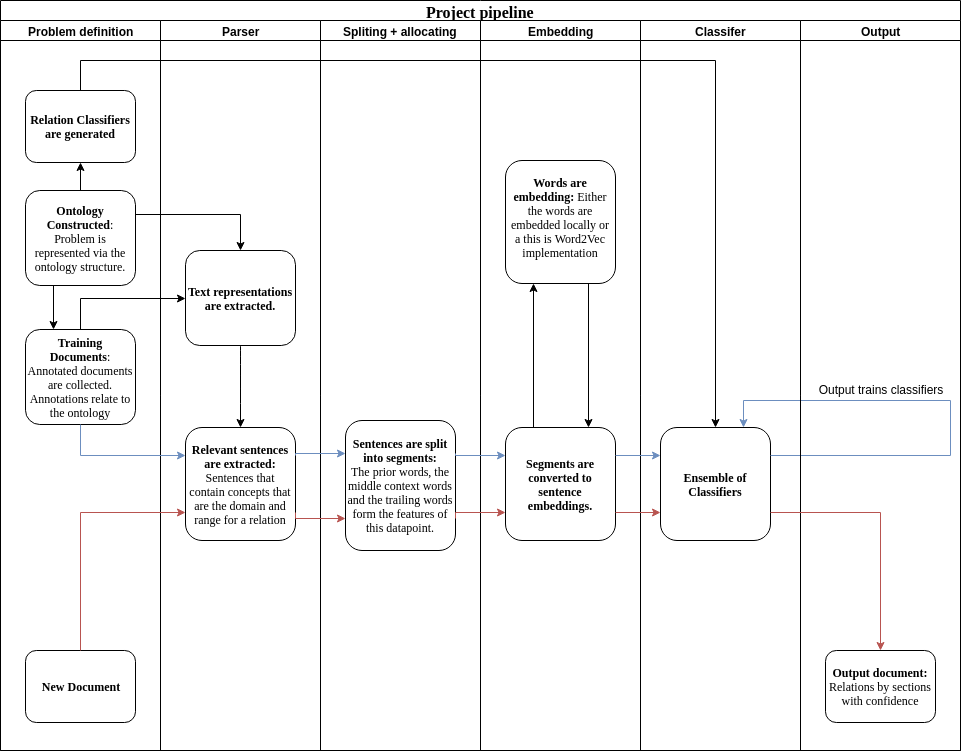
\includegraphics[scale=0.4,natwidth=610,natheight=642]{Project-pipeline.png}
    \caption{Initial visualisation of the expected path through the system}
\end{figure}

\subsection{Original Specification}

Primarily, the system I envisioned was rather more self-contained. It was my intention to interact with the model and functionality through a single object. However, as development began, it became clear that for the intended use, a whole variety of objects could prove as useful supporting objects and structures. Though the package provides many objects to interact with, the goal of maintaining an intuitive method of interaction has been preserved.

\subsubsection{Structure}

The project shall be a python package that enables the creation of the project’s relation classifier. The classifier a simplistic API primarily offering functionality to train and predict on annotated sets. A classifier will take as part of its constructor the ontology that describes the domain. For training, a set of annotated document objects will be taken along with their targets. The inputs to the object shall be in the form of an ontology object/file and a collection of annotated sentences/paragraphs.

\subsubsection{Ontology}

The ontology provides information about the entities and relations contained within the domain. Additionally, it indicates a hierarchy of entities to allow for cascading of relations. e.g. Person drives vehicle can be cascaded to Paul drives BMW. This helps ensure the document is relatively small and simplistic, facilitating development. It provides a powerful tool for the expansion of relations over the domain in a deterministic manner without losing information while being as general or specific as the user intends. Following suit, as a concept can relate to any arbitrary construct, the concept itself will be able to identify if it is expected to appear within a text, and with what representation. This will ensure that relations can cascade correctly, but, the relation extractor will not find to be true relationships between concepts that are not desired. Relations will allow the user to indicate various properties of the relationship, one such property is self-referencing. Though a relation holds between People, the relation does not ever hold for the same person to person.

\subsubsection{Technique}

Classification is to be performed by an ensemble of multilayer perceptron algorithms, similar to those expressed in M. Surdeanu et al (2007). Each classifier shall be tasked with determining the confidence of a particular relationship expressed within the ontology. They shall take as inputs tokens of a sentence that will be anchored around the entities. The number of inputs of a classifier shall be determined by K and shall express the number of context words around the pair to include. An input shall be the words before the first entity, the words between the pair of entities, and the words following the second entity. The entities themselves do not need to be included as they are assumed by the classifier. The classifier can then operate on any combination of entities within the ontology that inherit from the entities of the relationship, allowing one classifier to correctly evaluate many entity pairings. For situations where a single passage has the potential to exhibit multiple relations between concepts, each relation will be classified in turn. The confidence of their prediction will be used to indicate which of the relationships shall indeed hold. Additionally, as the classification of each relationship happens independently from one another, the system shall allow the user to programmatically introduce relations into its evaluation at any time. At such time, additional classifiers will be generated and the model will extend to handle these relations.

\subsubsection{Training}

Training the system focus on paragraphs/sentences that contain entities that can express relationships found within the ontology. For entity pairs, the relations are identified and the classifiers responsible for representing them are found. Words within a sentence shall be tokenized, and the features shall be expanded to include their respective Part of speech tags.

\subsubsection{Prediction}

The system is to return a collection of relations found along with the  segments of text they originated from, their index in the text, and their confidence. During the evaluation section, the input document will be subjected to various refinement processes designed to minimise error. Spelling will be corrected, co-referencing shall be conducted and entities inserted.

\subsection{Development Methodology}

For the development of my project, I adhered to the agile development style as best a singular individual can, by breaking down the aspects of the project into various collections of functionality. I was able to iteratively add features according to their priority in the context of the scope of the project. Along with the development of these features, I spent time ensuring each parts validity by writing unit tests. It was critical to ensure each stage was thoroughly tested to reduce the overhead of resolving issues caused by service integration.

It was important to ensure that the project was correct and complete at each stage of addition of additional features. I intend to continue to develop this package to include other tools and operations for the extraction/generation of information. Each feature added was accompanied by unit and service tests to ensure validity.

\subsection{Deviations from the original Specification}

During the course of development, I identified that certain assumptions where either not sensible or detracted from the potential of the system. Following from this I editted the original specification and listed below these changes.

\subsubsection{Structure}

Overall the structure of the solutions is consistent with the original envisioned system. The solution is a Python package that contains the functionality to generate and manipulate ontologies and the relation extractor itself. A variety of tools also accompany the package for the convenience of users, most importantly document objects. The relation extractor has itself become a valid ontology object that maintains, along with the concepts and relations of the domain, an ensemble of relation classifiers. The input has become solely the training documents objects that help process raw text into a machine-readable manner.

\subsubsection{Ontology}

The ontology functionality is as originally states, though functionality is divided into the Concept, Relation objects. The ontology maintains this information and provides an expansive interface for interaction with the information.

\subsubsection{Technique}

The parameter ``K" (number of words of context) has been removed as it is based on the premise that individual words are to form the features of any given data point and be passed to the classifiers. Due to the variability of sentence length and large occurrence of missing features, the method of tokenizing the context around an entity pair has changed. The training documents along with a collection of external texts are used to produce a model for word embedding, which in turn is used to perform sentence embedding in the context around pairings. The features are then the features of the sentence embedding alleviating the original issues. The total context window has become individual sentences themselves. This has meant a new parameter has been introduced ``S" which refers to the size of the word embedding vector, with a default value of 300, as suggested by research conducted by Google \cite{tang2014learning}.

Other than this change, the relation model operates as originally specified. The concepts themselves are not passed to the model as they are considered interchangeable with any other concepts the relationship connects, as expressed by the ontology. As such, its semantic value shouldn’t and doesn’t impact classification.

\subsubsection{Training}

Training is solely conducted through the use of the training document object. The training documents are to include the text source, and all the data points the text expresses with annotations of the points into three various classifications. The classification: Positive, an example of when a relationship holds; Negative, an example of when the relation is shown to be not true, not present; and Null, when the concepts of a relationship are present, but the context doesn’t offer any information about the relationship. An example:

\noindent``Kieran has lived in France for 2 years now, but he still doesn’t know French"

If considering the relationships ``born in", ``lives in" and ``speaks". Kieran living in France is a positive instance, Kieran being born in France, is a null instance, and Kieran speaks French is a negative instance. Though it can be inferred that Kieran was not born in France, (if he is older than 2), performing inference is not within scope. The purpose of the extraction is only to extract semantic relationships that are present in the text itself. Since there is no context that gives any indication that the relation ``born in" holds, it is considered a null instance.

Training documents can be created programmatically, or via the Annotation Document object, that allows a user to annotate a document from the command line. Given that an ontology of the domain already exists, all the potential data points from a text source can be extracted, and the user can classify each data point, iteratively generating a training document.

\subsubsection{Prediction}

Similar to how one trains a relation extraction model, the method to predict on a source is to generate a document object with the source as its content. These documents are passed into the model and once the predictions have been made, the document objects are updated to contain the data points found. The document has a collection of points for every sentence, ordered accordingly. Each data point contains information about the original text, the matches made, the context, and ultimately the predicted class and its probability. Points that were predicted as null are no present as they yield no information.

My original intention was that the document object was to be responsible for the refinement of its content before evaluation, however, these processes also require training to work effectively. Spelling corrections are handled by a statistical model that is trained on the contents of the training document \cite{whitelaw2009using}\cite{choudhury2007difficult}. The spelling model is then included during the cleaning of a sentence to alleviate issues. 

I have also decided not to remove stopping words, as though my experiments, examples indicated that the removal will definitely lead to incorrect classification. ``Kieran can speak English", ``Kieran cannot speak English", ``Kieran doesn’t speak English" will all collapse to ``Kieran speak English" via the removal of stopping words thus, they are required.

Anaphora resolution was not implemented within the system due to the complexity of the field, which ultimately reduces the system’s capacity to recall instances. This limitation is confined to cross sentence referencing only, the contextual information innately contains co-referencing information, thus, the system is still able to learn these relationships. The system currently is positioned to allow for the quick adoption of an anaphora resolution method in future iterations.

\section{Design and Implementation}

I designed the solution in the style of a python package such that the system would be easy to include into systems that expand multiple platforms, and to be able to make use of the scientific packages that are popular in python.

\subsection{Ontology}

The ontology object is fundamentally a programmatic implementation of the ontology concept expressed within philosophy. It is a form of Knowledge representation that encompasses the collection and organisation of world knowledge. This knowledge is the backbone of my relation extraction implementation as it guides the processing of input documents and the generation of relation classifiers. Similarly to the philosophical ontology, it expressed information by declaring what things exist (concepts), and how they interact(relationships).

\subsubsection{Concept} \label{concept}

The concept object represents a singular \textit{thing} in the domain covered by the ontology. A concept can relate to any imaginable construct, including an idea, a location and a time. A concept encapsulated the relevant information necessary to express its part in the ontology and describes how it might interact. Within the project itself, a concept could be considered a bare-bones realisation of this ideal. Concepts are responsible for generating a structure of knowledge and permitting a simplistic method of relation expansion with I will discuss in the following section. Concepts are uniquely identified with a name, and store information about parent and child concepts, possible attributes (properties) and their visibility in the text.\\

Family membership is a method of implicitly specifying the relation commonly referred to as ``is a". This relation indicates that ``child's" concepts can operate in the space of their parents indistinguishably. The concept object holds this information and provides convenient functions for the use of this information and the comparison with other concepts.

\subsubsection{Relationship}

A relationship defines one of the potentially many forms of interaction between two concepts. Information is encapsulated implicitly in the definition of the relation, it does not in itself relate to any particular \textit{thing}, but rather, the interaction of \textit{things}. The relation object within the project abstractly represents a collection of semantic relationships that can be formed between concepts. Fundamentally, the relation object is to represent semantic relations that exhibit the same textual representation. As such, it is not subject to the conventional uses of philosophical relations. A relation object instead is used to describe a collection of related semantic relations, that can be referred to as consistent with one another within the domain. The relation object is responsible for maintaining this collection and nothing further.\\

A relation object maintains a collection of concept to concept pairings which represent the concepts it is expressing a relationship for. These pairs are referred to within the system as domain-target pairings, implicitly indicating that relationships are directional.\\ 


[Person, Business, Country] pays [Person, Business, Country]\\


Above is an example of a relationship object. The structure captures the domain concepts to the left within square braces, the relation name in the middle, and the target concepts on the right with square braces. It expresses the idea that the concepts ``Person", ``Business" and ``Country" can in some form ``pay" one another. The relation is as we would expect, the embodyment of the process of passing legal tender from one to another, and intuitively we know that this relationship exists between all of the concepts listed. Fundamentally, we know that despite the varying implications, the manner in which each of these pairings would be found within a text is extremely similar. In fact, we would expect that for a sentence that expresses the relationship between one pairing of the sentence, would express the relationship for any pairing if the concepts were interchanged.\\

The relationship as shown indicates how one might define a bidirectional relation, the number of connections this relation object actually expresses is the product of the domain-target sets. In doing so, all concepts can ``pay" themselves. The ability to self-reference has additional benefits when you consider the fact that ``Person" is a concept that encompasses a large collection of other concepts. As expressed within the section \ref{concept}, our ontology may contain concepts such as ``Kieran", ``Ben" and ``Luke", all of which express the ``is a" relationship with ``Person". The structure formed from the ``is a" relationship allows this simple relation definition to cascade to include child concepts as domains and targets. This process results in pays(``Kieran", ``Ben") to be a valid instance of this relationship. In total, this compact definition can, in fact, express 36 different relationship instances.\\

In the event that the relationship holds for most but not all of the instances that would be generated from the product of the two sets, the relationship can, in fact, define sets of domain-target pairs. Taking the example shown above, if we imagine that there can never be a relationship ``Country pays Person", then the current definition of the relationship is wrong. The original cross-product functionality is maintained as it greatly diminishes complexity, and instead, the instances become the sum of the sets of instances expressed in domain-target sets. The valid relation definition is:\\

\noindent Pays :

[Person, Business, Country] - [Business, Country]

[Person, Business] - [Person]\\

Something important to note for this example is that the conventional manner in which a country ``pays" an individual is typically through a specific process which is well defined, and accompanied by its own conventions in natural language. Though this would imply that the pairs are not as interchangeable as previously stated, it actually forms the reasoning as to why distinguishing this difference isn’t necessary.\\

Considering the relation expressed in originally, with a single set for the domain and target. If there is a convention in natural language that specifically expresses how countries pay other countries, then, this convention is not used to express the payment between other concepts such as people. Following this, the convention shall not appear within an examinable text in the domain expressing the relationship between other concepts. In kind, distinguishing the interactions separately is not necessary as they won’t appear, and the classifier can learn this separation without issue.\\

A counter argument may be that, though the convention should not appear, natural language is filled with mistakes and misuse, subsequently, it is possible that these events are found. I would argue that this doesn’t undermine any assumptions made when constructing the relationship. Fundamentally, human persons that are confronted with these issues are able to interpret the sentiment of the statement and form their own classification regardless of breaks in the convention. As such the sentiment of the convention is the predominant factor required to inform the decision. This leads to a design decision within the relation extraction process highlighted in section \ref{extractor}.\\

If there is a more critical departure of the textual representations, the relation's concepts can be split, or a new relationship can be generated. Situations like this are typically self-evident.

\subsubsection{Ontology}

The ontology class is the data structure that holds and manipulates the concept and relation objects. Exposing a simplistic interface to allow for programmatic addition and removal of concepts and relationships. The ontology class is responsible for ensuring the validity of its contents, propagating relationships down the ``is a" relationship structure and subscribing new concepts to relations where applicable. Concepts and Relations hold references to one another that are governed and owned by the ontology object, this ensures parallelisation of similar ontologies without conflict. Additionally, it provides the functionality to save and load a construction along with a number of other convenient functions. It acts as the main access point for concepts and relations.

\subsection{Documents}

Documents refer to a textual source of information. For the relation extraction, document objects wrap around content and provide the system with functionality to efficiently extract and use information.

\subsubsection{Datapoint}

All documents maintain a collection of data points, the data points record the all relevant information about a potential semantic relationship found within a snippet of text. A data point contains information about the relationship instance, the text where the relation was assumed to be present, and a breakdown of the snippet into context pockets around the concepts. For data points involved in training, an annotation value is also present. Additionally, the data point object maintains values for the context embeddings of each context pocket, the prediction value and the probability associated with that prediction.

\subsubsection{Annotator Document and the Prediction Document}

Within the project, a document that is to be treated as a source for prediction is simply referred to as a document. To avoid ambiguity, I will refer to said documents as Prediction documents (PD). Both the Annotator Document (AD) and the PD provide a simple method of interaction with a data source. Their primary responsibility is to process the source such that it is easier to interact with. A PD on generation simply extracts the contents of the source. Upon prediction, an ontology is passed that expresses the domain that document is to be reviewed within. The PD is then responsible for iteratively finding potential data points that may be present within the source.\\

The text representations of the concepts within the ontology form a collection of patterns used to introspectively query the source. The source is broken down first by paragraph, and then by sentence as dictated by the Document Operations module. Within each sentence, non-overlapping concepts are extracted. For each pair of concepts, the ontology is queried for all relationship that can form between them. All of this information is used to generate a collection of data points. In this state, the document can then be passed into the Relation extractor, as the data points to predict on have been set.\\

The AD extends the PD and provides a user with the ability to annotate the data points rather than having the prediction applied via the relation extraction system. Currently, the AD has a simplistic command line interface that allows for the generation of training documents off the back of the PD. Despite being a rudimental implementation, the AD allows the user to quickly generate training documents from an arbitrary text source. The responsibilities of this class are expected to greatly increase in future iterations of the system.

\subsubsection{Training Document}

The training document is a structure to contain already annotated data points. Its primary function is to hold the data points and provide a quick method of identifying concept text representations and yielding feature information. The structure of the document is less relevant as its purpose is to provide examples. 

\subsubsection{Document Operations}

Most of the operations conducted throughout the system and generic and stateless, as a result, the Document Operations (DO) module contains a number of convenience functions to process text snippets when applicable.\\

The most notable function provided by the DO is that conversion of a text snippet into an embeddable format. Referred to as ``cleanSentence", the method removes grammar, expands words and resolves spelling mistakes. Spelling is corrected using a simple implementation of Google’s spelling correction method. The method is essentially a model using probability theory to predict the spelling of a word not seen via the occurrence of candidate spellings in a large text corpus. During the training process of the Relation Extraction Model, the training documents are used along with text collections to train the spelling corrector model.

\subsection{Relation Extractor} \label{extractor}

The relation extractor is responsible for the functionality that makes prediction possible. Due to its dependence on the ontology for it to operate, the extractor is an extension of the ontology class and inherits its functionality. This provides much more granular control and flexibility. During initialization, an ensemble of neural network classifiers is generated which correspond one for one with the relationships expressed in the ontology. At this stage, the word embedding model is instantiated.\\

Word embedding is the blanket term for techniques that maps words and phrases as part of a set of vocabulary into a continuous vector space with greatly reduced dimensionality. This allows the words in the context snippets of a data point to be expressed as a vector of real numbers. The semantic information of a word is what is being represented, as it is believed that the company of a word gives it its definition. As such, Word embedding is a supervised method where large corpora of text are examined to find correlations between various words. The embedder can learn the semantic meaning of the words given the context they appear in.\\

During the training process, the contents of the training documents are passed into the word embedding model to enable a better fit of the domain-specific contextual semantic meanings of words. After training of the word embedding model is complete, the data points are extracted from the training documents and sorted according to their relationship. Each data point has its context snippets embedded according to the sentence embedding function.\\

Sentence embedding is a continuation of word embedding, that represents an entire collection of words in a single real vector. An additional consideration of sentence embedding is the information regarding the ordering of the words as this fundamentally alters the semantic definition of a sentence. The relation extractor generates a sentence embedding as the sum of its word embeddings. By default, the relation extractor uses an exponential monotonic function as a multiplier for each word embedding as a method of include positioning information for the embedding of the context.\\

With the training data points embedded, the Relation extractor trains each of the relation instance models in parallel (according to the number of threads parameter set). The Relation instance model takes the three embedded context snippets as its input only, excluding the concept representations. This is due to the previously stated interchangeability of the concepts in theory, and also to alleviate the semantic differences in the concepts themselves from the semantic construction of the surrounding context.\\

After the Relation Extractor has been fitted, prediction works in a similar vein to training. The Relation Extractor generates a thread to execute each document, which first passes a reference of the extractor's ontology to the document so that the document can generate its data points. Each of the data points is then embedded according to the sentence embedding function and passed to the relation instance model for classification. The predicted classification and its associated probability are then stored in the data point object itself and passed back to the document. After all of the PDs have been classified, they are passed back to the user's call and the entire process has been concluded. By having the operation of the relation extractor as written, the interface is limited to the initialisation of the extraction, the calling of the fit method, and the calling of the predict method.\\

The parameters of the system are limited to ensure that interacting with the system is as simple as possible. As the extractor extends the ontology, it uses the same default arguments to initialise its internal values. It may either be loaded from file, started fresh, or become a clone of another ontology that is passed in. The extractor is then responsible for the management of the word embedding model. This may be passed in as a user constructed model, to be used by the extractor, or the values around its embedding size and worker rate can be given. This allows the extractor to generate the word embedding model in the event that one isn't saved within the package and the user has not provided one. Finally, the extractor exposes the hidden layer structure of the relation models, and their corresponding alpha value as parameters into the system. These are the parameters that cross validation aims to tune.

\subsection{Supporting packages}

The system makes use of the following packages in its computation. These form the requirements of the system when implemented withing another process, or on another platform.

\subsubsection{Gensim}
Gensim is a framework for fast vector space modelling that provides functionality to perform topic modelling, document indexing and general information retrieval. They provide the word embedding implementation that is used within the relation extraction. Their intuitive interfaces expose memory-independent algorithms with respect to corpus size, that can be optimised for multicore implementations and distributed systems equally. They provide lots of utility and are the most popular method of generating word embeddings within Python.

\subsubsection{Sklearn}
Sklearn is a library built upon SciPy and contains a set of well tested and popular machine learning and data mining algorithms. Sklearn provides a simple and efficient toolset along with many methods of analysis. The SKlearn implementation of the Neural Network was used inside the relation instance model, to be able to classify the data points. These packages are very popular and well maintained themselves which provides validity and assurance to the code.

\section{Experimental Investigation and Analysis}

It is the aim of any application to yield good performance, quickly, while being inexpensive to operate. Within the field of information extraction, relation extraction follows the same trend. The performance of a system is measured by system's ability to recall relationships from within a text, and its ability to precisely predict their classifications. Due to the interactions of these measures (low recalls correlates with high precisions) the combined score ``F1" is conventionally used to describe the quality of a relation extraction method.\\

The recall rate is the number of relevant relations that have been identified over the number of relations present within a text the dataset expressed. The system will yield additional relationships, but the measure is of the known relations, excluding these points from the comparison. Precision is the measure of the number of correctly classified relations out of the relations that were recalled correctly.\\

For the use of the relation extractor, an ontology must declare the concepts and relationships that are to be extracted from the text. During the analysis, I identified that the recall rate is negatively affected by the undefined set of concept representations. The systems ability to adapt to various domains is an aim of the project, this will be identified by looking at the precision and recall of the system over a number of datasets and comparing the results collected with that of the method implemented.

\subsection{Drug-related adverse effects from medical case reports}

\cite{gurulingappa2012development} has developed a benchmark for relation extraction using information from MEDLINE. MEDLINE contains more than 1.5 million medical case reports. In order to restrict the scope of the corpus to drug-related adverse events, a PubMed 12 search with drug therapy and adverse effect as MeSH \cite{lowe1994understanding} terms was performed limiting the language to English. The text option was chosen to be abstract in order to eliminate the documents with the only title and no abstract text.\\

This process retrieved nearly 30,000 documents from PubMed out of which 3000 documents (referred to as ADE corpus) were randomly selected for the annotation and benchmarking purposes. A corpus of 3000 annotated documents is believed to be substantially large to support the development and validation of information extraction systems. Sentences from the corpora were split into two classifications positive and negative. The negative set encapsulates null and negative instances as a by-product.\\

The performance of the sentence classification framework was evaluated using 10-fold cross-validation \cite{kohavi1995study}. During the cross-validation experiments, the discriminative capability of the classifier to correctly distinguish between the informative and non-informative sentences was measured using Precision, Recall, and F 1 score over the class Positive as a criterion. A MaxEnt model trained with simple features such as words in the sentence resulted in a good classification performance. Removal of stop-words degraded the performance of classification.

\begin{center}
 \begin{tabular}{||c c c c||} 
 \hline
 Model & Precision & Recall & F1 \\ [0.5ex] 
 \hline\hline
 InfoGain & 0.778 & 0.711 & 0.774 \\ 
 \hline
 Naive Bayes & 0.91 & 0.08 & 0.14 \\
 \hline
 MaxEnt & 0.75 & 0.64 & 0.70 \\
 \hline
\end{tabular}
\end{center}

A small caveat to the results posted is that the precision score calculated by \cite{gurulingappa2012development} is the precision value of the points that were correctly recalled, not over the space of points. This is what leads to Naives Bayes high precision value, as its extraction method is responsible for removing challenging data points and offers simply points to classify. That being said, my method has produced a high precision score over the dataset and yielding the greatest F1 score. Cross validation was found the best parameter settings to be: Hidden layer size (300, 6, 3), alpha = 1.4384498882876659e-09

\begin{figure}
\centering
\includegraphics[width=8cm]{ADEHiddenLayer.pdf}
\caption{The metric values for the ADE cross validation, the effect of hidden layer changes for static alpha}
\end{figure}

\begin{figure}
\centering
\includegraphics[width=8cm]{ADEAlpha.pdf}
\caption{The metric values for the ADE cross validation, the effect of alpha value changes for static structure}
\end{figure}

\subsection{Classification of Semantic Relations between Nominals}

\cite{girju2007semeval} relate to authors present an evaluation task designed to provide a framework for comparing different approaches to classifying semantic relations between nominals in a sentence. This is part of SemEval, the 4 th edition of the semantic evaluation event previously known as SensEval. The dataset expressed 8 different relationships:\\

\begin{figure}[h]
    \centering
    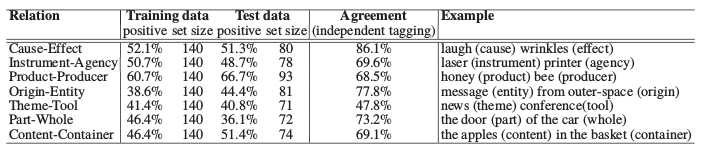
\includegraphics[scale=0.6]{WordVec.png}
    \caption{Relation description and WordVec statistics during the generation of the dataset}
\end{figure}

The data set that \cite{nastase2006learning} created used relation labels, part-of-speech tags and WordNet sense annotations, to facilitate its classification. \cite{moldovan2004models}\cite{girju2005semantics} gave the annotators an example of each phrase in a sentence along with WordNet senses and position of arguments. During the testing phases of the algorithms, due to the fact that many of the systems wanted to exploit a number of these kinds of information, the testing was broken down into 4 distinct categories. Each category referred to a different combination of additional WordNet information.


\begin{center}
 \begin{tabular}{||c c c c||} 
 \hline
 Model & Precision & Recall & F1 \\ [0.5ex] 
 \hline\hline
 InfoGain & 0.655 & 0 & 0 \\ 
 \hline
 UDC-FC & 0.661 & 0.667 & 0.664 \\
 \hline
 ILK & 0.605 & 0.695 & 0.638 \\
 \hline
 UMELB-B & 0.615 & 0.55.7 & 0.578 \\
 \hline
 UC3M & 0.482 & 0.403 & 0.431 \\ [1ex] 
 \hline
\end{tabular}
\end{center}

\begin{figure}
\centering
\includegraphics[width=12cm]{SEMHiddenLayer.pdf}
\caption{The metric values for the SemEval cross validation, the effect of hidden layer changes for static alpha}
\end{figure}

\begin{figure}
\centering
\includegraphics[width=12cm]{SEMAlpha.pdf}
\caption{The metric values for the SemEval cross validation, the effect of alpha value changes for static structure}
\end{figure}

For our implementation, only the annotations from the dataset were extracted and used, thus we are comparing the results of my Relation Extraction Model against their category ``A", which relates to the minimal amount of additional information. Unfortunately none of the data points expressed in the test set had a domain-target pairing that matched one expressed in the training set, as a consequence, non of the data points could be recalled. The precision score listed showes the precision of the model if 100\% recall is enforced. As we can see from the results, the method was able to achieve an extremely competitive precision score across the dataset. My implementation was within a single percentage point away from the best method. During cross validation, the method performed best with the parameters: Hidden layer shape (300,50,20), alpha 1.4384498882876659e-09

\subsection{Evaluation Conclusions}

There were a number of challenges that were presented by the datasets that I had to tackle. While translating the information into a format that my model could process, I realised that I was having to make a few assumptions about the use case, that didn’t align with the spirit of my method. The fundamental aspect of my classification model is its efficient use of an ontology that expresses the domain. The ontology construct is intended to help guide relation extraction by declaring potential relationships and provide the information necessary to identify potential data points within a text before they have been sent to the prediction model. As part of the processing of the datasets, I had to generate an ontology from the training data that expressed the domain. For both datasets, the number of relationships that were being examined was predetermined as part of the task/innate to the problem. However, the set of concepts that appeared, and their respective representations, were not known beforehand, and in SemEval case, where generated on the fly. As no information was provided about the concepts structure, I used the training data to generate a single layer ontology that simply listed the concepts that were present. This results in an ontology that is first, incomplete in its definition, and secondly, without any intelligent design. This was not in the spirit of the method. The ontology is intended to be far more expressive and conclusive.\\

In light of this, I draw a conclusion that the recall rate of the system could, in fact, be modelled statistically. As the representations of the concepts are what is used to extract potential data points. No datapoint that contains a concept representation not expressed in the training set can be extracted. Ergo, the recall rate for a testing set is equal to the sum of the set of representations in the testing set intersected with the set of representations in the training set, over the sum of representations in the testing set.

\begin{equation}
recall = \frac{C_{te} \cap C_{tr}}{C_{te}}
\end{equation}\\

As a result, when looking at the recall rates of the system via the malformed ontologies, we can see why the recall rates are low. In ADE’s case, the concepts that appear within the negative examples are simply not specified, and when considering the size of the negative set (9452) in comparison to the positive set (1425), you can see cause for its low recall score. The concepts within the SemEvals dataset are simply far too expensive with very little reuse. \\

The method by which I generated recall scores was to produce a document that contained its content, the text snippets of each data point as a sentence. Though it may have lacked, correct recall, there were still some potential data points that were found, that were not expressed in the original dataset. Though these don’t play into the metric scores, I felt it necessary to point out that as these datasets don’t specify null instances, the classifiers always indicating the presence of a relationship for the data points it finds.\\

What is promising, is that due the extraction model’s disregard for the true representation of the concepts within the data point it is predicting, its ability to predict is un-hindered, thus, precisions is not at all affected by this issue. The cross validation also showed something interesting, for the SemEval dataset, the greater the complexity of the relation models the greater the precision. This is likely due to the complexy of the problem and the nature of the language being used. The relations were vague in their definition and the language was flamboyant and erratic. To accurately model this behaviour, the model needed to be more complex. For the ADE dataset, the language was very formal and precise, with a clear definition within the relation, as such, even a very small small structure was able to distinguish between the positive and negative instances.


\section{Solution Evaluation}

When looking at the aims and objectives of the project, I believe that the system is a success. Using the system is extremely simplistic, as shown in the examples \ref{examplescript}. Generating an ontology, generating some training and testing documents and then prediction via a relation model can be done in less than 100 lines. Most importantly, the model provides competitive performance in the space matching precision scores of supervised and semi-supervised methods. Additionally, the package provides a host of supporting functions and data types to be able to allow a user to interact with their data and the model efficiently and effectively. The model also sports only a few parameters and allows the user to provide their own word embedding model if they would like.\\

There are a number of examples of the flexibility of the system. The model is able to generate and maintain a collection of relation prediction models that are independent, allowing for the addition of new relationship into the system on the fly. As the concept representation doesn’t impact prediction, adding additional concepts to the domain or range of a relation doesn’t affect the model's performance. This would indicate that the model is also rather extendable, allowing for the addition of more concepts and relationships during operation.\\ 

As the major aspects of the system are threaded and separated into multiple processes, the relation extraction model is able to scale well on a variety of platforms. Via the method of data point extraction, no preprocessing is done where it needn’t, ensuring that redundant information is removed as soon as possible. The operation of the model is relatively quick, the loading and training of the word embedding model and the relationship model is workable in a matter of seconds.\\

The ontology object not only facilitates the relation extraction but is useful for encapsulating knowledge even as a separate instance. The package provides a great deal of functionality for the manipulation, construction and comparison of an ontology, and is position greatly for improvements in future iterations of the system.\\

During the evaluation process, its challenges associated with recall indicated an issue that may present itself to potential users. For domains where representations of the concepts are far to large a set to confidently record, extraction will ultimately suffer as a consequence. As result, its implementation will likely have to be accompanied by a form of entity recognition to be able to appease large and unruly domains.


\section{Conclusion}

I have developed a system for the extraction and classification of semantic relationships in the form of a python package. The development was driven by the consideration that the package had a purpose, that users would be intending to build off of the insights that can be gained from the system. As such, the system facilitates a users ability to quantify a domains knowledge, through the use of an ontology, and extract only the relevant information. I have designed it such that its insights can be programmatically interpreted and included, such that the method can be integrated into a preexisting system with minimal effort. I have examined and made use of the techniques expressed in a number of related literature pieces, choosing to implement the system as an ensemble of neural network classifiers. The principal patterns that the models are attempting to learn are the semantic patterns held by the relation that can be derived from the context around the concepts/entities.\\

The method has shown to be effective in its operation achieving competitive precision against a number of implementations on 2 datasets. Unfortunately, the analysis indicated that performance was heavily tied to the collection practices, that can limit the model in sparse environments. The design of the system has been shown to be flexible to changing and inhospitable domains, extendable to various problems, and scalable across a plethora of platforms.


\subsubsection{Limitations}

A requirement of the system is that the ontology expresses all occurrences of possible concepts and relationships before examining any of the training data. A problem that I have identified during the processing of both datasets was the fact that it may not be a realistic expectation to assume that the user knows of all the ways in which a concept will be expressed. Text representations are extracted from the training data and add to the patterns used to extract data points from PD, however, these training documents are likely not able to provide examples of every possible text representation of the potentially expansive ontology structure. Subsequently, the method’s ability to recall instances is limited to the percentage of representation coverage in the ontology and the training documents.\\

Currently, due to the absence of an anaphora resolution method, recall is affected by relationships that use co-referenced concepts. As the current method of data point generation is pattern matching on the text representations, the system is incapable of matching these co-referencing relations if the original concept is not apart of the sentence. The current method does work for resolving inner sentence co-referencing but in a subpar manner.\\

``Kieran can speak English rather well, but he has never lived in England."\\

This example of an inner match highlights how the system currently operates. It is clear that two relationships are present within the text, Kieran speaks English, and not Kieran lived\_in ``England". A human person would interpret the second relationship between the pronoun ``he" and ``England", however, due to the pattern matching, the context extracted for this data point would be the entire middle context as it matches the instance Kieran and the instance England across the text. As this kind of extraction is consistent throughout the training and prediction process, the system shall learn how to correctly predict those points, however, this unintentionally adds additional variety to how the relationship may occur which negatively impacts the classification. Secondly, as the relationship may be expressed but not throughout the sentence, the context in the middle of the sentence has very little or nothing do to do with the relation further harming classification.\\

In the event that anaphora resolution was introduced, this would likely exacerbate another issue. For sentences that contain multiple references to the same concept, it is possible for multiple data points to be generated with the same relation instances but varying context snippets.\\

\noindent``Kieran can speak English well, Kieran has always spoken it well."\\

Though it is correct to extract both data points for comparison, a human would interpret the data point that spans ``English well, Kieran" as an incorrect point. The issue arises as the method by which a data point is selected is based on the probability of its classification. In turn, the incorrect point can be selected if its classification is made with great certainty. This will result in a malformed explanation of why the relationship is said to be held. Though this is a relatively small inconvenience for the user rather than a flaw, a larger issue arises when a context is malformed enough to provide a different classification. As the malformed context will likely not be used during training of the relation, it is possible that the malformed point will not only be classified with greater probability, but with an incorrect class. Subsequently, negatively impacting the perceived performance of the classifier. As stated, this issue is likely to be exacerbated as the anaphora resolutions are used to find additional concepts within the text.\\


\subsubsection{Future work}

The predominant problems facing the current version of the system relate to the method by which data points are extracted from the PD. For dealing with issues related to incomplete text representations, incorporating a method of entity recognition during the training phase may allow the extractor to improve upon its recall rates. Additional functionality can be added to allow text representations that are classified as a concept within the ontology, with a confidence above a threshold to be added to the ontology for future use.\\

Leveraging the \cite{exploringVarious} method for the identification of entity types may provide a simplistic method of incorporating some co-referencing resolution. A result would be that the PD documents would be responsible for maintaining two versions of a source's content.\\

As the method by which the context is embedded is a combination of the word embeddings, words that form phrases are unable to provide the correct semantic interpretation. A method of identifying phrases, and in turn, generating a phrase embedding for a collection of words, would likely yield an improvement in classification.\\

Adapting the document objects to maintain their contents is a compressed form may help ensure that the memory requirement of the system is kept to a minimum. The document objects would then be responsible for expanding the content when needed and yielding small parts at a time. Additionally, The document objects could also be expanded to handle a greater variety of encodings. Though this will come with greater challenges for the embedding and training aspects of the system, providing greater flexibility is also a requires aspect of a system.\\

During the testing of the ADE corpus, it was apparent that the concept ``Dosage" was an imperial unit with a particular form. An adaptation of the concept text representation procedure would likely be beneficial in capturing concepts that may have an infinite number of representations. Using concept representation patterns would likely increase recall rates as a simple rule is being used to expand the potential pool.\\

The current system can stand to benefit greatly from an additional abstraction of the embedding protocols. A consistent interface between these functions and the main system would allow for development or introduction of other methods or systems to fulfil this role in affecting the current system. Furthermore, it can inform the spelling corrector module of its insights.\\

The sentence embedding function should be editted such that the it's asymptote and gradient are parameters to be able to tune. I have the feeling that for different corpa, a different implementation may yield performance gains.

\subsubsection{Personal Reflection}

Personally, I am very happy with the state of the system and am proud that with the results its have been able to achieve. I had the preconceived notion that the basic implementation of my sentence embedding would lead to subpar results, but I have been pleasantly surprised. The system as a whole has lots of potential for future development which I am sure will lead to quicker training cycles and improved classifications.  

\bibliography{SRE}

\newpage
\section{Appendix}

\subsection{Example ontology and Example script} \label{examplescript}


\includegraphics[]{ExampleOntology.pdf}

\includepdf[pages=-,scale=0.9,pagecommand={}]{scriptExample.pdf}

\begin{figure}
\centering
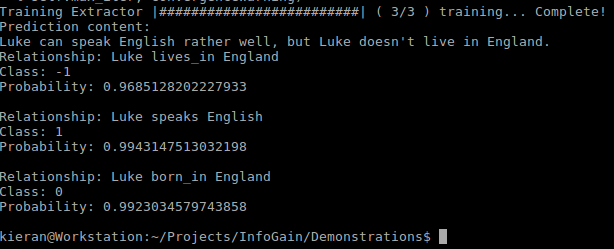
\includegraphics[scale=0.8]{Example.png}
\end{figure}


\end{document}